\addtocounter{section}{24}
\section{Höhere Ableitungen und \person{Taylor}-scher Satz} \proplbl{section_taylor} \setcounter{equation}{0}

\begin{boldenvironment}[Vorbetrachtung] Sei $X$ endlich dimensionaler, normierter Raum über $K$ (d.. Vektorraum über $K$ mit Norm $\Vert \,\cdot \Vert$, $\dim X =l\in\mathbb{N}$).
	
	Offebar sind $X$ und $K^l$ isomorph als Vektorraum, schreibe $X\cong K^l$, z.B. $X = L(K^n,K^m)\cong K^{m\cdot n}$.
	
	Für $g:D\subset K^n\to X$, $D$ offen, kann man die bisherigen Resultate bezüglich der Ableitung übertragen. $g'(x)\in L(K^n, X)$ heißt Ableitung von $g$ im Punkt $x\in D$, falls \begin{align*}
		g(x + y) = g(x) + g'x() y + o(\vert y\vert), \;y\to 0
	\end{align*}
\end{boldenvironment}
	
\begin{*definition}[zweite Ableitung]
Betrachte nun $f:D\subset K^n\to K^m$, $D$ offen, $f$ \gls{diffbar} auf $D$. Falls $g:= f':D\to L(K^n, K^m) =: y_1$ \gls{diffbar} in $x\in D$ ist, heißt \begin{align}
	f''(x) := g'(x)\in L(K^n, Y_1) = L\big( K^n, \underbrace{L(K^n, K^m)}_{\cong K^{m\times n}}\big)
\end{align}
\begriff{zweite Ableitung} von $f$ in $X$.
\end{*definition}

\begin{underlinedenvironment}
	Offenbar gilt dann: \begin{align}
	\notag f'(x + y) &= f'(x) + f''(x)y + o(\vert y \vert),\; y\to 0
	\intertext{bzw.}
	\proplbl{taylor_definition_hoehere_ableitung_zwei}
	f'(x+y)\cdot z &= f'(x)\cdot z + \underbrace{\big( \underbrace{f''(x)\cdot y}_{\in K^{m\times n}} \big) z}_{\in K^m} + o(\vert y \vert)\cdot z\quad\forall z\in K^n
	\end{align}
\end{underlinedenvironment}

\begin{boldenvironment}[Interpretation]
	Betrachte $f''(x)$ als kubische bzw. $3$-dimensionale "`Matrix"' (heißt auch \emph{Tensor} 3. Ordnung).
	
	\emph{beachte:} Ausdruck für $f''(x + y)\cdot z$ ist jeweils linear in $y$ und $z$.
\end{boldenvironment}

\begin{boldenvironment}[Frage] höhere Ableitungen, d.h. von $f'':D\to L(K^n, Y_1)$ usw.
	
	Offenbar: \begin{align*}
		g_2&:= L(K^n, Y_1) = L\big(K^n, L(K^n K^m)\big) \cong L(K^n, K^{m\times n}) \cong L(K^n, K^{m\times n}) \cong K^{m\cdot n^2}\\
		g_3&:= L(K^n, Y_2) \cong L(K^n, K^{m\cdot n^2}) \cong K^{k\cdot n^3}
	\end{align*}
	Endlich dimenionale, normierte Räume, man kann rekursiv $\forall k\in \mathbb{N}$ definieren: \begin{enumerate}[label={(\roman*)}]
		\item (Räume)
		
		\begin{tabularx}{\linewidth}{l@{\ }c@{\ }l@{\ }X}
			$Y_0$ & = & $K^n$ &  mit $\vert\,.\,\vert$ \\
			$Y_{k+1}$ &  :=  & $L(K^n, Y_k)$ & mit Standardnormen $\Vert A\Vert_{k+1} = \sup\limits_{\vert z \vert \le 1} \Vert Az\Vert_{Y_k}$ (vgl. Satz 13.8),
		\end{tabularx}
		analog zu oben ist $Y_k\cong K^{m\cdot n^k}$, $Y_k$ normierter Raum
		
		\item (Ableitungen)
		
		\begin{tabularx}{\linewidth}{l@{\ }c@{\ }X}
			$f^{(0)}$ & := & $f:D\subset K^n\to K^m$, $D$ offen.\\
		\end{tabularx}
		Falls $f^{(k)}:D\to Y_k$ \gls{diffbar} in $x\in D$ heißt \[ f^{(k+1)}(x) := \left( f^{(k)} \right) (x)\in L(K^n, Y_k)  \]
		\begriff{$(k+1)$-te Ableitung} von $f$ in $x$. (\emph{beachte:} $f^{(1)}(x) = f'(x)$)
		
		Somit gilt: \begin{align}
			f^{(k)} (x + y) = f^{(k)}(x) + f^{(k+1)}(x) \cdot y + o(\vert y \vert) \;(\in Y_k), \;y\to 0
		\end{align}
	\end{enumerate}
\end{boldenvironment}

\begin{*definition}[$k$-fach differenzierbar]
	$f$ heißt \begriff{$k$-fach differenzierbar} (auf $D$), falls $f^{(k)}$(x) existiert $\forall x\in D$.
	
	$f$ heißt $k$-fach stetig \gls{diffbar} (auf $D$) oder $C^k$-Funktion, falls $f$ $k$-fach \gls{diffbar} und $f^{(k)}:D\to Y_k$ stetig.
	
	$C^k(D, K^m) := \{ f:D\to K^m\mid $f$ \text{ $k$-fach stetig \gls{diffbar} auf $D$} \}$
\end{*definition}

\begin{underlinedenvironment}[Hinweis]
	Falls $f^(k)(x)$ existiert $\Rightarrow$ $f^{(k-1)}$ stetig in $X$  (vgl. \propref{diffbar_impl_stetig})
\end{underlinedenvironment}
\begin{boldenvironment}[Speziafall $n=1$]
	$f:D\subset K\to K^m$\\
	\begin{tabularx}{\linewidth}{r@{$\;$}l@{$\,$}c@{$\,$}X}
	$f'(x)$ & $\in Y_1 = L(K, K^n)$ & $\cong$ & $K^m$ \\
	$f''(x)$ & $\in Y_2 = L(K, Y_1)$ & $\cong$ &  $L(K, K^m)\cong K^m$
	\end{tabularx}
	Allgemein: $f^{(k)}(x) \in Y_k = L(K, Y_{k-1}) \cong L(K, K^m)\cong K^m$, d.h. für $n=1$ kann $f^{(k)}(x)$ stets als $m$-Vektor in $K^m$ betrachtet werden.
\end{boldenvironment}

\begin{example}
	Für $f:\mathbb{R}\to\mathbb{R}$ mit $f(x) = x\cdot \sin x$\\ \begin{tabularx}{\linewidth}{r@{\ \ }r@{\ }c@{\ }l}
		$\Rightarrow$ & $f'(x)$ & = & $\sin x + x\cdot \cos x $ \\
		$\Rightarrow$ & $f''(x)$ & = & $\cos x + \cos x - x \sin x = 2 \cos x - x \sin x$ \\
		$\Rightarrow$ & $f'''(x)$ & = & $-3\sin x - x\cos x$ usw.
	\end{tabularx}
	\begin{center}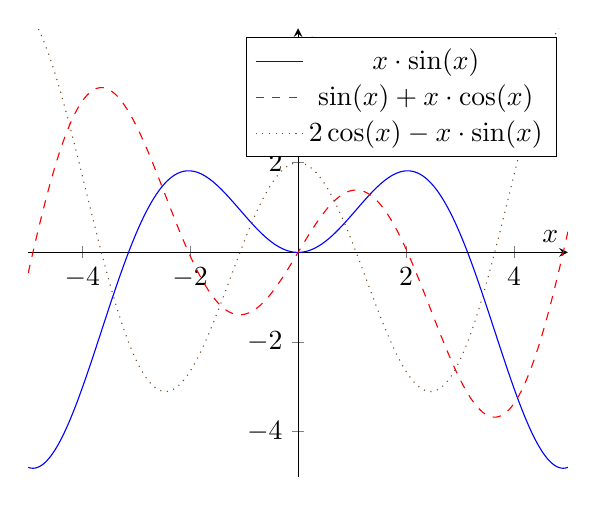
\begin{tikzpicture}
		\begin{axis}[
		xmin=-5, xmax=5, xlabel=$x$,
		ymin=-5, ymax=5, ylabel=$y$,
		samples=400,
		axis y line=middle,
		axis x line=middle,
		]
		\addplot+[mark=none] {x*sin(deg(x))};
		\addlegendentry{$x\cdot\sin(x)$}
		\addplot+[mark=none, dashed] {sin(deg(x))+x*cos(deg(x))};
		\addlegendentry{$\sin(x)+x\cdot\cos(x)$}
		\addplot+[mark=none, dotted] {2*cos(deg(x))-x*sin(deg(x))};
		\addlegendentry{$2\cos(x)-x\cdot\sin(x)$}
		\end{axis}
		\end{tikzpicture}\end{center}
\end{example}

\begin{example}
	sei $f:\mathbb{R}_{> 0}\to\mathbb{R}^2$ mit $f(x) = \binom{x^3}{\ln x}$. \begin{align*}
		\Rightarrow\;f'(x) &= \begin{pmatrix}
			3x^2 \\ \frac{1}{x}
		\end{pmatrix} & \Rightarrow\; f''(x) &= \begin{pmatrix}
			6x \\ -\frac{1}{x^2}
		\end{pmatrix} & \Rightarrow\; f'''(x) &= \begin{pmatrix}
			6 \\ \frac{2}{x^3}
		\end{pmatrix}
	\end{align*}
\end{example}

\begin{example}
	Sei $f:\mathbb{R}\to\mathbb{R}$ mit \begin{flalign*}
		f(x) &= \begin{cases}
			x^3 & x\ge 0 \\
			-x^3 & x < 0
		\end{cases} &
	\end{flalign*}
	Folglich
	\begin{align*}
		\Rightarrow\; f'(x) &= \begin{cases}
			3x^2 \\ -3x^2
		\end{cases} & \Rightarrow \; f''(x) &= \begin{cases}
			6x \\ -6x
		\end{cases}
	\end{align*}
	$\Rightarrow$ $f'''(0)$ existiert nicht, d.h. $f\in C^2(K, \mathbb{R})$ aber $f\notin C^3(\mathbb{R},\mathbb{R})$
\end{example}

\begin{example}
	\proplbl{tayler_hoehere_ableitungen_beispiel_4}
	Sei $f:\mathbb{R}\to\mathbb{R}$ mit \begin{align*}
		f(x) &= \begin{cases}
			e^{-\frac{1}{x}} & x > 0 \\
			0 & x\le 0
		\end{cases}
	\end{align*}
	$\Rightarrow$ $f^{(k)}(x)$ existiert $\forall x\in\mathbb{R}$, $k\in\mathbb{N}$ mit $f^{(k)}(0) = 0$ $\forall k$, d.h. $f\in C^k(\mathbb{R},\mathbb{R})$ $\forall k\in \mathbb{N}$.
	
	Man schreibt auch $f\in C^\infty(\mathbb{R},\mathbb{R})$
\end{example}

\begin{boldenvironment}[Räume $Y_k$] $=L(K^n, Y_{k-1}) \cong K^{m\times n^k}$.
\end{boldenvironment}

Für $A\in Y_k = L(K^n, Y_{k-1})$ und $y_1, \dotsc, y_k\in K^n$ gilt:

\begin{tabularx}{\linewidth}{l@{$\,$}l@{$\,$}X}
$A\cdot y_1$ & $\in Y_{k-1}$ & $= L(K^n, Y_{k-2})$,\\
$(A y_1)\cdot y_2$ & $\in Y_{k-2}$ & $ = L(K^n, Y_{k-3})$ \\
& $\vdots$ & \\
$(\dotsc (A y_1) y_2) \dotsc \cdot y_k)$ & $ \in Y_0$ & $ = K^m$
\end{tabularx}

Ausdrücke links sind offebar linear in jedem $y_j\in K^n$ separat, $j=1\dotsc,k$

\begin{*definition}[$k$-lineare Abbildung]
Betrachte \begin{align*}
X_k &:= L^k(K^n, K^m) \\
&:= \{ B: \underbrace{K^n \times \dotsc \times K^n}_{\text{$k$-fach}} \to K^m \mid y_j \to B(y_1, \dotsc, y_k) \text{ linear für jedes $j=1,\dotsc,k$ }\}
\end{align*}
$B\in X_k$ heißt \begriff{$k$-lineare Abbildung}. $X_k$ ist Vektorraum.
\end{*definition}

\begin{example}
	Für 3-lineare Abbildung $B\in L^3(\mathbb{R},\mathbb{R}^2)$ mit \begin{align*}
		B(x,y,z) &= \begin{pmatrix}
			xyz \\ (x+y) z
		\end{pmatrix}
	\end{align*}
	ist z.B. \emph{nicht} linear als Abbildung auf $\mathbb{R}^3$.
\end{example}

\begin{proposition}
	\proplbl{taylor_ismomorphismus_yk_xk}
	Für $k\in\mathbb{N}$ ist $I_k:Y_k\to X_k$ mit \begin{align}
		\proplbl{taylor_isomorphismus_yk_xk_eq}
		(I_k A)(y_1, \dotsc, y_k) &:= \left( \dotsc \big( (A y_1)  y_2\big) \dotsc y_k\right) \quad\forall A\in Y_k,\;y_j\in K^n,\;j=1,\dotsc,k
	\end{align}
	ein Isomorphismus bezüglich der Vektorraum-Struktur (also $X_k\cong Y_k$).
	
	\begin{underlinedenvironment}[Hinweis]
		Somit kann $f^{(k)}(x)$ auch als Element von $X_k$ betrachtet werden, d.h. $f^{(k)}(x)\in X_k = L^k(K^n, K^m)$
		
		Damit wird z.B. \eqref{taylor_definition_hoehere_ableitung_zwei} zu \begin{align}
			f'(x+y)\cdot z &= f'(x)\cdot z + f''(x)\cdot(y,z) + o(\vert y \vert)\cdot z\quad\forall z\in K^n
		\end{align}
		und für $n=1$ gilt \begin{align*}
			f^{(k)}(x) (y_1, \dotsc, y_k) &= \underbrace{f^{(k)}(x)}_{\in K^m} \cdot \underbrace{y_1 \cdot \dotsc y_k}_{\mathrlap{\text{Produkt von Zahlen}}} \quad\forall y_j \in K
		\end{align*}
	\end{underlinedenvironment}
\end{proposition}

\begin{proof}
	$I_k$ offenbar linear auf $Y_k$, $I_k$ injektiv, denn $I_k(A) = 0$ \gls{gdw} $A = 0$
	
	Zeige mittels Vollständiger Induktion: $I_,$ surjektiv.
	
	\begin{tabularx}{\linewidth}{@{}lX}
		\emph{IA:} & Offenbar ist $X_1 = Y_1$ und $I_1 A = A$ $\Rightarrow$ $I_1$ surjektiv \\
		\emph{IS:} & Sei $I_k$ surjektiv und wähle beliebiges $B\in X_{k+1}$.
		
		Setze $\tilde{B}_{y_1} := B(y_1, \,\cdot\, ,\dotsc,\,\cdot\,)\in X_k$ $\forall y_1\in K^n$, $\tilde{B}\in L(K^n, X_k)$
	\end{tabularx}
	\zeroAmsmathAlignVSpaces*
	\begin{flalign}
		\proplbl{taylor_ismorphismus_yk_xk_beweis_eq_6}
		\phantom{\emph{\texttt{IA:}}\ \ \ }\;&\Rightarrow \;\; A:=I_k^{-1} \tilde{B}\in L(K^n, Y_k) = Y_{k+1} & \\
		\notag&\; \begin{alignedat}{2}\Rightarrow\;\;(I_{k+1}A)(y_1,\dotsc,y_{k+1}) &\overset{\eqref{taylor_isomorphismus_yk_xk_eq}}{=} \left( \dotsc\big( (Ay_1)y_2 \big) \dotsc y_{k+1}\right) &\;=\;& \big(I_K(Ay_1)\big) (y_2, \dotsc, y_{k+1})\\
		& \overset{\eqref{taylor_ismorphismus_yk_xk_beweis_eq_6}}{=} (\tilde{B}y_1)(y_2, \dotsc, y_{k+1}) &\;=\;& B(y_1, \dotsc, y_{k+1})
		\end{alignedat}
	\end{flalign}
	\begin{tabularx}{\linewidth}{@{}ll@{\ \ }X}
		\phantom{\texttt{IS:}} & \ $\Rightarrow$ & $B = I_{k+1} \cdot A$ $\Rightarrow$ $I_{k+1}$ surjektiv
	\end{tabularx}
	$\Rightarrow$ $I_k$ Isomorphismus
\end{proof}

\begin{boldenvironment}[Norm] in $X_k$, $Y_k$: für $A\in Y_k$ folgt durch rekursive Definition \begin{align}
		\notag
		& \left(\dotsc\left(  \left( A \frac{y_1}{\vert y_1\vert}\right) \frac{y_2}{\vert y_2 \vert} \right) \dotsc \frac{y_k}{\vert y_k \vert} \right) \le \Vert A\Vert_{Y_k} \quad \forall y_j\in K^n,\; y_j\neq 0 \\
		\proplbl{taylor_hoehere_ableitungen_norm}
		\Rightarrow \;\;& \left( \dotsc \big( (Ay_1) y_2 \big) \dotsc y_k \right) \le \Vert A \Vert _{Y_k} \vert y_1\vert \vert y_2\vert \dotsc \vert y_k\vert \quad \forall y_1\,\dotsc,y_k\in K^n 
	\end{align}
	Norm für $A\in X_k = L^k(K^n, K^m)$: \begin{align*}
		\Vert A\Vert _{X_k} := \sup \{ \vert A(y_1, \dotsc, y_k)\vert \mid y_j \in K^n,\; \vert y_j\vert \le 1 \}
	\end{align*}
	Analog zu \eqref{taylor_hoehere_ableitungen_norm} folgt für $A\in X_k$:\begin{align}
		\proplbl{taylor_hoehere_ableitung_abschaetzung_norm}
		\vert A(y_1, \dotsc, y_k)\vert \le \Vert A\Vert_{X_k} \vert y_1 \vert \cdot \dotsc \cdot \vert y_k\vert \quad\forall y_j\in K^n
	\end{align}
\end{boldenvironment}

\begin{proposition}
	Mit Isomorphismus $I_k: Y_k\to X_k$ aus \propref{taylor_ismomorphismus_yk_xk} gilt: \begin{align*}
		\Vert I_(A)\Vert_{X_k} &= \Vert A \Vert_{Y_k} \quad\forall A\in Y_k
	\end{align*}
\end{proposition}
\begin{proof}
	Selbststudium / ÜA
\end{proof}

\begin{remark}
	\proplbl{taylor_partielle_ableitung_isomorphismus_bemerkung}
	$\Vert f^{(k)}(x)\Vert$ unabhängig davon, ob man $f^{(k)}(x)$ als Element von $X_k$ oder $Y_k$ betrachtet.
\end{remark}

\subsection{Partielle Ableitungen}
Sei $X=(x_1, \dotsc, x_k)\in K^n$; d.h. $x_j\in K$, $e_1, \dotsc, e_k$ die Standard-Einheitsvektoren

\begin{boldenvironment}[Wiederholung]
	Partielle Ableitung $f_{x_j} (x) = \frac{\partial}{\partial x_j}f(x) = D_{x_j} f(x)$ ist Richtungsableitung $f'(x, e_j) = D_{e_j} f(x) \in L(K, K^m)$.
\end{boldenvironment}

\begin{*definition}[partielle Ableitung]
	Nenne $f_{x_1}(x), \dotsc, f_{x_1}(x)$ \uline{partielle Ableitung }\begriff[partielle Ableitung!]{1. Ordnung} von $f$ in $X$
	
	Für $g:D\to X$ definieren wir die partielle Ableitung $\frac{\partial}{\partial x_j} g(x) = g_{x_j}(x)\in L(K, X)$ analog zu \propref{richtungsableitung}:\begin{align}
		g(x + t\cdot e_j) &= g(x) + g_{x_j}(x)t + o(t), \;t\to 0,\;t\in K
	\end{align}
	Für $g=f_x:D\to L(K, K^m)$ ist dann $g_{x_j}\in L\big( K, L(K, K^m) \big)$. Für $g = f_{x_j}: D\to L(K, K^m)$ ist dann $g_{x_j}\in L(K, L(K, K^m)) \cong L^2(K, K^m)\cong K^m$
	die  \begriff{partielle Ableitung} $f_{x_i x_j} (x)$ von $f$ in $x$ nach $x_i$ und $x_j$.
	
	Andere Notation: $\frac{\partial^2}{\partial x_j x_i} f(x), D_{x_i x_j} f(x), \dotsc$
	
	Die $f_{x_i x_j}(x)$ heißen \uline{partielle Ableitung} \begriff[partielle Ableitung!]{2. Ordnung} von $f$ in $x$.
	
	Mittels Rekursion \begin{align}
	\proplbl{taylor_partielle_ableitung_definition_10}
		f_{x_{j_1}\dots x_{j_k}}(x) := \frac{\partial}{\partial x_i} f_{x_{i_1} \dots x_{j_k}}
	\end{align}
	erhält man schrittweise die \uline{partielle Ableitung} \begriff[partielle Ableitung!]{der Ordnung $k\in\mathbb{N}$} von $f$ in $x$: \begin{align*}
		f_{x_{j_1}\dots x_{j_k}}(x) = D_{x_{j_1}\dots x_{j_k}} f(x) = \frac{\partial ^k}{\partial x_{j_k} \dots \partial _{x_{j_1}}} f(x) \in L^k(K, K^m)
	\end{align*}
	
	Berechnung durch schrittweises Ableiten von $x_{j_1}\to f(x_1, \dotsc, xn)$, $x_{j_2}\to f_{x_{j_1}}(x_1, \dotsc, x_n)$ usw.
\end{*definition}

\begin{example}
	\proplbl{taylor_partielle_ableitungen_beispiel_9}
	Sei $f:\mathbb{R}^2\to\mathbb{R}$ mit $f(x,y) = y\sin x$ $\forall x,y\in\mathbb{R}$ und \begin{align*}
		f_x(x,y) &= y\cos x & f_y(x,y) &= \sin x\\
		f_{xx}(x,y) &= -y\sin x & f_{yy}(x,y) &= 0 \\
		f_{xy}(x,y) &= \cos x & f_{yx}(x,y) &= \cos x
	\end{align*}
	
	\begin{boldenvironment}[Beobachtung]
		$f_{xy}(x,y) = f_{yx}(x,y)$
	\end{boldenvironment}
\end{example}

Abkürzende Schreibweise: \begin{align*}
	f_{x_j x_j x_j}(x) &= \frac{\partial^3}{\partial x_j \partial x_j \partial x_j} f(x) = \frac{\partial^3}{\partial x_j^3} f(x) \\
	f_{x_i x_j x_i x_l x_l}f(x) &= \frac{\partial}{\partial x_l^2 \partial x_j^2 \partial x_i} f(x)
\end{align*}
\begin{*definition}[\person{Hesse}-Matrix]
Für $m=1$ (d.h. $f:D\subset\mathbb{R}^n\to K$) ist 
\begin{align*}
	\begin{pmatrix}
		f_{x_1 x_1}(x) & \dotsc & f_{x_1 x_n}(x) \\
		\vdots & & \vdots \\
		f_{x_n x_1}(x) & \dotsc & f_{x_n x_n}(x)
	\end{pmatrix} &=: \mathrm{Hess}(f)
\end{align*}
die \begriff{\person{Hesse}-Matrix}, die alle partiellen Ableitungen 2. Ordnung enthält.
\end{*definition}

\begin{example}
	\proplbl{taylor_partielle_ableitung_beispiel_10}
	Sei $f=(f_1, f_2): \mathbb{R}^2\to\mathbb{R}^2$ mit \begin{align*}
		\begin{pmatrix}
			f_1(x_1, x_2) \\ f_2(x_1, x_2)
		\end{pmatrix} = \begin{pmatrix}
			x_1^2 x_2 \\ x_1 x_2 + x_2^2
		\end{pmatrix}
	\end{align*}
	Folglich \begin{align*}
		f_{x_1}(x_1, x_2) &= \begin{pmatrix}
			2 x_1 x_2 \\ x_2
		\end{pmatrix} & f_{x_2}(x_1, x_2) &= \begin{pmatrix}
			x_1^2 \\ x_1 + 2 x_2
		\end{pmatrix}
	\end{align*}
	und \begin{align*}
		\begin{pmatrix}
			2 x_1 x_2 & x_1^2 \\ x_2 & x_1 + 2x_2
		\end{pmatrix}
	\end{align*}
	ist die \person{Jacobi}-Matrix sowie
	\begin{align*}
		\textrm{Hess}(f_1) &= \begin{pmatrix}
			2 x_2 & 2 x_1 \\ 2x_1  & 0
		\end{pmatrix} & \textrm{Hess}(f_2) &= \begin{pmatrix}
			0 & 1 \\ 1 & 2
		\end{pmatrix}
	\end{align*}
	Anschaulich: alle partiellen Ableitungen 2. Ordnung bilden eine 3D Matrix.
\end{example}

\begin{boldenvironment}[Frage]
	Zusammenhang von $f^{(k)}(x)$ mit partiellen Ableitungen?
\end{boldenvironment}

\begin{theorem}
	\proplbl{taylor_partielle_ableitung_zusammenhang_hoehere_ableitung}
	Sei $f:D\subset K^n\to K^m$, $D$ offen, $x\in D$. Dann \begin{enumerate}[label={(\alph*)}]
		\item Falls $f^{(k)}(x)$ existiert, dann existieren alle partiellen Ableitungen der Ordnung $k$ in $x$ und \begin{align}
			\proplbl{taylor_partielle_ableitung_zusammenhang_hoehere_ableitung_eq}
			f_{x_{j_1}\dotsc x_{j_k}}(x) = f^{(k)}(x)(e_{j_k},\dotsc,e_{j_1})
		\end{align}
		\item \proplbl{taylor_partielle_ableitung_zusammenhang_hoehere_ableitung_b}
		Falls alle partiellen Ableitungen $f_{x_{j_1}\dots x_{j_k}}$ der Ordnung $k$ für alle $y\in B_r(x)\subset D$ existieren und falls diese stetig sind \\
		\ \ $\Rightarrow$ $f$ ist $k$-fach \gls{diffbar}, d.h. $f^{(k)}(x)$ existiert.
	\end{enumerate}
\end{theorem}

\begin{remark}
	\propref{taylor_partielle_ableitung_zusammenhang_hoehere_ableitung} \ref{taylor_partielle_ableitung_zusammenhang_hoehere_ableitung_b} ist ein wichtiges Kriterium zur Prüfung der \gls{diffbar}keit, $k$-te Ableitung kann dann mittels \eqref{taylor_partielle_ableitung_zusammenhang_hoehere_ableitung_eq} bestimmt werden.
\end{remark}

\begin{proof}
	Jeweils mittels vollständiger Induktion nach $K$ ausgeführt:\begin{enumerate}[label={\alph*)},topsep=\dimexpr-\baselineskip/2\relax]
		\item basiert auf \propref{richtungsableitung_vollstaendige_reduktion} 
		\item basiert auf \propref{mittelwertsatz_existenz_partieller_ableitung}
	\end{enumerate}
\end{proof}

\begin{example}[nochmal \propref{taylor_partielle_ableitung_beispiel_10}]
	$f^{(2)}(x) = f''(x) \in L^2(\mathbb{R}^2, \mathbb{R}^2)$ existiert $\forall x=(x_1, x_2)\in\mathbb{R}^2$ nach \propref{taylor_partielle_ableitung_zusammenhang_hoehere_ableitung} und kann als Vektor von der \person{Hesse}-Matrix dargestellt werden: \begin{align*}
		f^{(2)} (x) = \begin{pmatrix}
			\textrm{Hess} f_1 \\ \textrm{Hess} f_2
		\end{pmatrix} = \begin{pmatrix}
			\begin{pmatrix}
				2 x_2 & 2 x_1 \\ 2 x_1 & 0
			\end{pmatrix} \\ \begin{pmatrix}
				0 & 1 \\ 1 & 2
			\end{pmatrix}
		\end{pmatrix}
	\end{align*}
	Was ist nun $f''(x)(y_1, y_2)$ für (Vektoren) $y_1$, $y_2\in\mathbb{R}^2$?
	\begin{align*}
		f''(x)(y_1, y_2) &= f''(x) \begin{pmatrix}
			\binom{y_{11}}{y_{12}}, \binom{y_{21}}{y_{22}}
		\end{pmatrix} = f^{(2)}(x) (y_{11} e_1 + y_{12}e_2, y_{21}e_1 + y_{22}e_2) \\
		&= y_{11}f''(x)(e_1,y_2) + y_{12}f''(x)(e_2,y_2)\marginnote{Linearität!} \\
		&= y_{21}y_{11}f''(x)(e_1,e_1) + y_{12}y_{21}f''(x)(e_2,e_1) + y_{11}y_{22}f''(x)(e_1,e_2) + y_{12}y_{22}f''(x)(e_2, e_2) \\
		& \overset{\eqref{taylor_partielle_ableitung_zusammenhang_hoehere_ableitung_eq}}{=} y_{11}y_{21} f''_{x_1 x_1}(x) + y_{12}y_{21}f_{x_1 x_2}(x) + y_{21}y_{22}f_{x_2 x_1}(x) + y_{12} y_{22} f_{x_2 x_2}(x) \;(\in\mathbb{R}^2) \\
		&= \begin{pmatrix}
			\langle (\mathrm{Hess} f_1)(x) y_1, y_2\rangle \\
			\langle (\mathrm{Hess}f_2)(x) y_1, y_2 \rangle
		\end{pmatrix} \in\mathbb{R}^2\quad\forall y_1, y_2\in\mathbb{R}^2
	\end{align*}
\end{example}

Analoge Rechnung liefert allgemein
\begin{conclusion}
	Für $f=(x_1, \dotsc, f_m):D\subset K^n\to K^m$, $D$ offen, es existieren alle $f^{(2)}(x)$ für $x\in D$. Dann \begin{align}
		f^{(2)}(x) (y_1,y_2) = \begin{pmatrix}
			\langle (\mathrm{Hess} f_1)(x) y_1, y_2\rangle \\ 
			\vdots\\
			\langle (\mathrm{Hess} f_m)(x) y_1,y_2\rangle
		\end{pmatrix} \in K^m\; \forall y_1, y_2\in K^n
	\end{align}
\end{conclusion}

\begin{remark}
	Für höhere Ableitungen wird die Darstellung $f^{(k)}(x)(y_1, \dotsc, y_k)$ allgemein mittels partiellen Ableitungen immer komplexer, wird allerdings auch selten benötigt.
\end{remark}

\begin{boldenvironment}[Frage:]
	Kann man die Reihenfolge bei partiellen Ableitungen vertauschen? (vgl. \propref{taylor_partielle_ableitungen_beispiel_9})
\end{boldenvironment}

\begin{example}
	Sei $f:\mathbb{R}^2\to\mathbb{R}^2$ mit\begin{align*}
		f(x,y) = \begin{cases}
			\frac{x^3y - xy^3}{x^2+y^2} & (x,y)\neq(0,0)\\
			0 & (x,y)=(0,0)
		\end{cases}
	\end{align*}
	und folglich \begin{align*}
		f_x(x,y) &= \begin{cases}
			\frac{y(x^4 + 4x^2 y^2 - y^4)}{(x^2 + y^2)^2} & \text{für }(x,y) \neq (0,0) \\
			\lim\limits_{t\to 0}\frac{f(t,0) - f(,0,)}{t} = 0 & \text{sonst}
		\end{cases}
	\end{align*}
	\begin{tabularx}{\linewidth}{l@{\ }l@{\ }c@{\ }r@{\ }l@{\ }X}
		
	insbesondere & $f_x(0,y)$ &=& $-y$& $\forall y\in \mathbb{R}$,& also $f_{xy}(0,0) = -1$ \\
	analog & $f_y(x,0)$ &=& $x$ & $\forall x\in\mathbb{R}$,& also $f_{yx}(0,0) = +1$
	\end{tabularx}
\end{example}

\begin{proposition}[Satz von \person{Schwarz}]
	\proplbl{taylor_partielle_ableitung_schwarz}
	Für $f:D\subset\mathbb{R}^n\to\mathbb{R}^m$, $D$ offen. Mögen die partiellen Ableitungen $f_{x_i}$, $f_{x_j}$, $f_{x_i x_j}$ auf $D$ existieren. Falls $f_{x_i x_j}$ stetig in $x\in D$
	\stepcounter{equation}
	\begin{flalign}
		\proplbl{taylor_partielle_ableitung_schwarz_eq}
		\Rightarrow\;\;& f_{x_j x_i}(x)\text{ existiert und } f_{x_i x_j}(x) = f_{x_j x_i}(x) &\marginnote{(13) fehlt}
	\end{flalign}
\end{proposition}

\begin{conclusion}
	\proplbl{taylor_partielle_ableitung_schwarz_folgerung}
	Sei $f:D\subset\mathbb{R}^n\to\mathbb{R}^m$, $D$ offen, $f$ $k$-fach \gls{diffbar} (d.h. $f\in C^k(D,\mathbb{R}^m)$) \\
	\ $\Rightarrow$ alle partiellen Ableitung bis Ordnung $k$ existieren und die Reihenfolge kann vertauscht werden.
\end{conclusion}

\begin{proof}[\propref{taylor_partielle_ableitung_schwarz_folgerung}]
	Existenz der partiellen Ableitung und deren Stetigkeit folgen aus \propref{taylor_partielle_ableitung_zusammenhang_hoehere_ableitung}, beliebige Vertauschung der Reihenfolge kann durch schrittweises Vertauschen von zwei "`benachbarten Veränderlichen"' erreicht werden.\\
	\ $\xRightarrow{\text{\cref{taylor_partielle_ableitung_schwarz}}}$ Behauptung
	
	Zur Veranschaulichung: \begin{align*}
		f_{x_3 x_1 x_2}(x) & \overset{\eqref{taylor_partielle_ableitung_definition_10}}{=} D_{x_2} f_{x_3 x_1}(x) \overset{\text{\cref{taylor_partielle_ableitung_schwarz}}}{=} D_{x_2}f_{x_1 x_3}(x) \overset{\eqref{taylor_partielle_ableitung_definition_10}}{=} f_{x_1 x_3 x_2}(x) \\
		& \overset{\eqref{taylor_partielle_ableitung_definition_10}}{=} (f_{x_1})_{x_3 x_2}(x) \overset{\text{\cref{taylor_partielle_ableitung_schwarz}}}{=} (f_{x_1})_{x_2 x_3}(x) \overset{\eqref{taylor_partielle_ableitung_definition_10}}{=} f_{x_1 x_2 x_3}(x)
	\end{align*}
\end{proof}

\begin{proof}[\propref{taylor_partielle_ableitung_schwarz}]
	\gls{obda} $m=1$. Fixiere $\epsilon > 0$ $\Rightarrow$ $\exists \delta > 0$ mit \begin{align*}
		x + s\cdot e_i + t\cdot e_j\in D\quad\forall s,t\in (-\delta,\delta)
	\end{align*}
	und
	\begin{align}
		\proplbl{taylor_partielle_ableitung_schwarz_beweis_15}
		\vert f_{x_i x_j}(x + s\cdot e_i + t\cdot e_j) - f_{x_i x_j}(x)\vert < \epsilon \quad\forall s,t\in(-\delta,\delta)
	\end{align}
	
	Definiere $\phi(s) := f(x + s\cdot e_i + t\cdot e_j) - f(x + s\cdot e_i)$ ist \gls{diffbar} auf $(-\delta,\delta)$ $\forall t\in (-\delta,\delta)$ \\
	\begin{tabularx}{\linewidth}{r@{\ \ }X}
	$\xRightarrow{\text{MWS}}$ & $\exists \sigma \in (0,s): \phi(s) - \phi(0) = \phi'(\sigma)s = \left(f_{x_i}(x + \sigma e_i + t e_j) - f_{x_i}(x + \sigma e_i)\right)s$ \marginnote{MWS = Mittelwertsatz, \propref{mittelwertsatz_mittelwertsatz}}\\
	$\xRightarrow{\text{MWS}}$ & für $t\to f_{x_i}(x + \sigma e_i + t e_j)$: $\exists \tau \in (0,t): \phi(s) - \phi(0) = f_{x_i x_j}(\underbrace{x + \sigma e_i + \tau e_j}_{=: \tilde{x}}) s t$ ($\sigma$, $\tau$ abhängig von $s$, $t$)
	\end{tabularx}
	Daher gilt:
	{\zeroAmsmathAlignVSpaces*\begin{align}
	\proplbl{taylor_partielle_ableitung_schwarz_16}
	\notag \left\vert\frac{\phi(s) - \phi(0)}{st} - f_{x_i x_j}(x)\right\vert &\le \underbrace{\left\vert\frac{\phi(s) - \phi(0)}{st} - f_{x_i x_j}(\tilde{x})\right\vert}_{=0} + \left\vert f_{x_i x_j}(\tilde{x}) - f_{x_i x_j}(x) \right\vert& \\
	&\overset{\eqref{taylor_partielle_ableitung_schwarz_beweis_15}}{<} \epsilon \quad\forall s,t\in(-\delta,\delta),\; s,t\neq 0&
	\end{align}}
	Wegen \begin{align*}
		\lim\limits_{t\to 0} \frac{\phi(s) - \phi(0)}{t} = \lim\limits_{t\to 0}\frac{f(x + s\cdot e_i + t\cdot e_j) - f(x + s \cdot e_i)}{t} - \frac{f(x + t\cdot e_j) - f(x)}{t} = f_{x_j}(x + s\cdot e_i) - f_{x_j}(x)
	\end{align*}
	folgt aus \propref{taylor_partielle_ableitung_schwarz_16} \begin{align}
		\proplbl{taylor_partielle_ableitung_schwarz_beweis_17}
		\left\vert \frac{f_{x_j}(x + s\cdot e_i) - f_{x_j}(x)}{s} - f_{x_i x_j}(x) \right\vert < \epsilon\quad \forall s\in (-\delta, \delta);\; s\neq 0
	\end{align}
	\ $\xRightarrow{\epsilon > 0}$ $f_{x_j x_i}(x) = \lim\limits_{s\to 0}\frac{f_{x_j}(x + s\cdot e_i) - f_{x_j}(x)}{s}\overset{\eqref{taylor_partielle_ableitung_schwarz_beweis_17}}{=} f_{x_i x_j}(x)$
\end{proof}

\subsection{Anwendungen}
\begin{boldenvironment}[Frage]
	Wann besitzt $fD\subset\mathbb{R}^n\to\mathbb{R}^{m\times n}$ eine Stammfunktion? (Vgl. \propref{stammfunktion}, \gls{obda} $m=1$)
\end{boldenvironment}

\begin{proposition}[notwendige Integrabilitätsbedingung]
	\proplbl{taylor_anwendung_integrabilitaetsbedinung}
	Sei $f=(f_1, \dotsc, f_n): D\subset\mathbb{R}^n\to\mathbb{R}^n$, $D$ Gebiet\marginnote{Gebiet: offen, zusammenhängend}, $f$ stetig \gls{diffbar}.
	
	Damit $f$ eine Stammfunktion $F:D\to \mathbb{R}$ besitzt, muss folgende \begriff{Integrabilitätsbedingung} erfüllt sein: \begin{align}
		\proplbl{taylor_anwendung_integrabilitaetsbedinung_eq}
		\frac{\partial}{\partial x_i} f_j(x) = \frac{\partial}{\partial x_j} f_i(x)\quad\forall x\in D,\; i,j=1,\dotsc,n
	\end{align}
\end{proposition}

\begin{remark}
	\eqref{taylor_anwendung_integrabilitaetsbedinung_eq} ist hinreichend, falls z.B. $D$ konvex (siehe Analysis 3)
\end{remark}

\begin{proof}
	$f$ habe Stammfunktion $F$ $\Rightarrow$ $F\in C^2(D)$
	
	\begin{tabularx}{\linewidth}{r@{\ \ }l@{\ }c@{\ }l@{\ }l}
	$\Rightarrow$ &$F_{x_j}(x)$& = &$f_j(x)$ &$\forall x\in D,j,i$ \\
	$\Rightarrow$& $F_{x_j x_i}(x)$& = &$\frac{\partial}{\partial x_i} f_j(x)$ & $\forall x\in D,i,j$ \\
	$\xRightarrow{\text{Schwarz}}$ & $F_{x_j x_i}(x)$ &=& \multicolumn{2}{l}{$F_{x_i x_j}(x) = \frac{\partial }{\partial x_j} f_i(x)$}
	\end{tabularx}
\end{proof}

\begin{example}
	Nochmal \propref{stammfunktion_beispiel_11} mit Parameter $\alpha\in\mathbb{R}$: \begin{align*}
		f(x,y) &= \begin{pmatrix}
			\alpha xy \\ x^2 + y^2
		\end{pmatrix}
	\end{align*}
	Betrachte die Ableitungen \begin{align*}
		\frac{\partial}{\partial y} f_1(x,y) &= \alpha x, & \frac{\partial}{\partial x} f_2(x,y) &= 2x
	\end{align*}
	$\xRightarrow{\eqref{taylor_anwendung_integrabilitaetsbedinung_eq}}$ $\alpha = 2$
\end{example}

\begin{proposition}
	Sei $f:D\subset\mathbb{R}^n\to\mathbb{R}$, $D$ offen und konvex, $f$ stetig \gls{diffbar}. Dann:\begin{enumerate}[label={\alph*)}]
		\item $f$ konvex $\Leftrightarrow$ $\langle f'(x), y- x\rangle \le f(y)f(x)$ $\forall x,y\in D$
		\item falls sogar $f\in C^2(D)$, dann: \begin{center}
			%@TODO zu definit linken
				$f$ konvex $\Leftrightarrow$ $f''(x) = (\mathrm{Hess} f)(x)$ positiv definit $\forall x\in D$
		\end{center}
	\end{enumerate}
\end{proposition}
\begin{proof}
	Vgl. Literatur
\end{proof}

\subsection{\person{Taylor}-scher Satz}
\begin{boldenvironment}[Ziel]
	Bessere Approximation als durch Linearisierung
\end{boldenvironment}

Verwende \begriff{allgemeine Polynome} $\phi:K^n\to K$ der Ordnung $k$, d.h. \begin{align}
	\phi(x) = a_0 + \sum_{i=1}^n a_i x_i + \sum_{i,j=1}^n a_{ij} x_i x_j + \dotsc + \sum_{j_1,\dotsc,j_k}^n a_{j_1\dots j_k} x_{j_1}\cdot\dots\cdot x_{j_k}
\end{align}
mit $a_0$, $a_j$, $a_{ij}$ $\in K$ gegebene Koeffizienten

\begin{boldenvironment}[Notation]
	 $f^{(k)}(x)(y,\dotsc,y) = f^{(k)}(x) y^k$
\end{boldenvironment}

\begin{boldenvironment}[Wiederholung]
	$f\in C(D)$: $f(x+y) = f(x) + o(1)$, $y\to 0$ \\
	$f\in C^1(D)$: $f(x+y) = f(x) + f(x)y + o(\vert y \vert)$, $y\to 0$
\end{boldenvironment}

\begin{theorem}[\person{Taylor}-scher Satz]
	 \proplbl{taylor_taylor}
	Sei $f:D\subset K^n\to K^m$, $D$ offen, $k$-fach \gls{diffbar} auf $D$, $x\in D$. Dann \begin{align}
		\proplbl{taylor_taylor_eq}
		f(x+y) = f(x) + \sum_{j=1}^{k-1} \frac{1}{j!} f^{(j)}(x) y^j + R_k(y)\quad\text{falls $[x,x+y]\subset D$,}
	\end{align}
	wobei\begin{align}
		\proplbl{taylor_taylor_restglied_eq_eins}
		\vert R_k(y)\vert \le \frac{1}{k!} \left\vert f^{(k)} (x + \tau y) y^k\right\vert \le \frac{1}{k!}\left\Vert f^{(k)} (x + \tau y)\right\Vert \vert y\vert^k
	\end{align}
	für ein $\tau = \tau(y)\in(0,1)$
	
	Für $K=\mathbb{R}$, $m=1$ gilt auch \begin{align}
		\proplbl{taylor_taylor_restglied_eq_zwei}
		R_k(y) &= \frac{1}{k!} f^{(k)}(x + \tau y) y^k
	\end{align}
	(\person{Lagrange} Restglied)
	
	Falls $f\in C^k(D, K^m)$ gilt: \begin{align}
		\proplbl{taylor_taylor_restglied_eq_drei}
		R_k(y) = \frac{1}{k!} f^{(k)}(x) y^k + o(\vert y\vert^k),\,y\to 0
	\end{align}
\end{theorem}

\begin{remark}
	Entscheidente Aussage in \propref{taylor_taylor} ist nicht \eqref{taylor_taylor_eq}, sondern die Eigenschaften des Restglieds (dies wird klein).
\end{remark}

\begin{proof}
	Sei $[x,x+y]\subset D$, definiere \begin{align*}
		R_K(y) = f(x + y) - f(x) - \sum_{j=1}^{k-1} \frac{1}{j!} f^{(j)}(x) y^j \quad\Rightarrow\eqref{taylor_taylor_eq}
	\end{align*}
	und definiere \begin{align*}\phi(t):= f(x + y) - f(x + ty) - \sum_{j=1}^{k-1} \frac{(1 - t)^j}{j!} f^{(j)}(x+ty) y^j - (1 - t)^k R_k(y)
	\end{align*}
	Offenbar $\phi(1) = 0 = \phi(0)$.
	
	Da $f$ $k$-fach \gls{diffbar}\\
	\begin{tabularx}{\linewidth}{r@{\ \ }X}
	$\Rightarrow$ & $\phi:[0,1]\to K^m$ $\mathbb{R}$-\gls{diffbar} auf $(0,1)$ mit
	\end{tabularx} {\begin{align}
		\proplbl{taylor_taylor_beweis_24}
		\notag\phi'(t) &= -f'(x + ty) \cdot y + \sum_{j=1}^{k-1}\left( \frac{(1 - t)^{j-1}}{(j - 1)!} f^{(j)}(x + ty) y^j - \frac{(1 - t)^j}{j!} f^{(j+1)}(x + ty) y^{j+1}\right) + k (1 - t)^{k - 1} R_k(y) \\
		& = - \frac{(1 - t)^{k-1}}{(k - 1)!} f^{(k)}(x + ty) y^k + k (1 - t)^{k-1} R_k(y)
	\end{align}}
	
	\begin{enumerate}[label={(\alph*)}]
		\item \marginnote{MWS = Mittelwertsatz, \propref{mittelwertsatz_mittelwertsatz}} $K=\mathbb{R}$, $n=1$: nach MWS $\exists \tau\in (0,1)$ und \begin{align*}
			0 = \phi(1) - \phi(0) = \phi'(\tau) \quad \xRightarrow{\eqref{taylor_taylor_beweis_24}} \eqref{taylor_taylor_restglied_eq_zwei}
		\end{align*}
		
		\item zu \eqref{taylor_taylor_restglied_eq_eins} mit $K=\mathbb{R}$: Sei $\psi(t) := \langle \phi(t), v\rangle$ für $v\in\mathbb{R}^n$ \\
		\begin{tabularx}{\linewidth}{r@{\ \ }X}
		$\Rightarrow$ & $\psi:[0,1]\to\mathbb{R}$ \gls{diffbar} auf $(0,1)$ mit $\psi'(t) = \langle \phi'(t),r\rangle$ \\
		$\xRightarrow{\text{MWS}}$ & $\exists \tau\in(0,1)$: $0= \langle \phi'(\tau), v\rangle$
		\end{tabularx}
		 {\begin{flalign}
		 	\proplbl{taylor_taylor_beweis_25}
		\qquad\Rightarrow\;\;&\langle R_K(y),v\rangle = \frac{1}{k!}\langle f^{(k)}(x + \tau y)y^k, v\rangle&
		\end{flalign}}
		mit $v = \frac{R_k(y)}{\vert R_k(y)\vert}$  ($\vert R_k(y)\vert \neq 0$, sonst klar) und es folgt
		\begin{align*}
			\langle R_k(y), v\rangle = \vert R_k(y)\vert = \left\langle \frac{1}{k!} f^{(k)}(x + \tau y) y^k, v\right\rangle \overset{\vert v \vert = 1}{\le} \frac{1}{k!} \left\vert f^{(k)}(x + \tau y) y^k\right\vert \quad\xRightarrow{\eqref{taylor_hoehere_ableitung_abschaetzung_norm}} \eqref{taylor_taylor_restglied_eq_eins}
		\end{align*}
		
		\item $K=\mathbb{C}$: identifiziere $\mathbb{C}^m$ mit $\mathbb{R}^{2m}$ und setzte $\phi(t) = \langle \phi(t), r\rangle_{\mathbb{R}^{2m}}$.
		
		Beachte:\begin{itemize}
			\item $\phi:[0,1]\to\mathbb{R}$, $\frac{\D}{\D t} \Re \phi_j(t) = \Re \frac{\D}{\D t}\phi_j(t)$ $\forall j$
			\item $\langle R_k(y), R_k(y)\rangle_{\mathbb{R}^{2m}} = \vert R_k(y)\vert_{\mathbb{C}^m}^2$
		\end{itemize}
		 und argumentiere wie in b)
			
		\item zu \eqref{taylor_taylor_restglied_eq_drei}: Setzte $R_k(y) = \frac{1}{k!}f^{(k)}(x) y^k + r_k(y)$ in \eqref{taylor_taylor_beweis_25}, $r = \frac{r_k(y)}{\vert r_k(y)\vert}$ (falls $r_k(y) \neq 0$)\\
		\begin{tabularx}{\linewidth}{r@{\ \ }X}
		$\Rightarrow$ & $\displaystyle\frac{\vert r_k(y)\vert}{\vert y \vert^k} \le \frac{1}{k!\vert y\vert^k} \left| \left( f^{(k)}(x + \tau(y)y) - f^{(k)}(x)\right)y^k\right| \overset{\eqref{taylor_hoehere_ableitung_abschaetzung_norm}}{\le} \frac{1}{k!} \left\Vert f^{(k)}(x + \tau (y)y) - f^{(k)}(x)\right\Vert \xrightarrow{y\to 0}0$,
		\end{tabularx}
		d.h. $r_k(y) = o(\vert y \vert^k)$, $y\to 0$
	\end{enumerate}
\end{proof}

\begin{*definition}[Taylorpolynom, Taylorentwicklung]
	Rechte Seite in \eqref{taylor_taylor_eq} ohne Restglied heißt \uline{Taylorpolynom}\begriff*[Taylor-!]{polynom} von $f$ in $x$ vom Grad $k-1$.
	
	\eqref{taylor_taylor_eq} heißt \uline{Taylorentwicklung}\begriff*[Taylor-!]{entwicklung} von $f$ in $x$.
\end{*definition}

\begin{conclusion}[\person{Taylor}-Formel mit partiellen Ableitungen]
	Sei $f:D\subset K^n\to K^m$, $d$ offen, $f$ $k$-fach \gls{diffbar} auf $D$, $x\in D$, $[c,c+y]\subset D$: \begin{align}
		\proplbl{taylor_taylor_partielle_ableitungen_eq}
		f(x + y) = f(x) = \sum_{l=1}^{k-1} \frac{1}{l!} \sum_{j=1}^n f_{x_{j_l}\dots x_{j_1}}(x) y_{j_1}\dots y_{j_l} + R_k(y),
	\end{align}
	wobei $y = (y_1, \dotsc, y_n)\in K^n$ (d.h $y_j\in K$ Zahlen).
\end{conclusion}

\begin{proof}
	Benutze \eqref{taylor_partielle_ableitung_zusammenhang_hoehere_ableitung_eq}
\end{proof}

\begin{remark}
	Falls alle partiellen Ableitungen von $f$ bis Ordnung $k$ existieren und stetig sind auf $D$ \\
	$\Rightarrow$ $f\in C^k(D)$ und \eqref{taylor_taylor_partielle_ableitungen_eq} (vgl. \propref{taylor_partielle_ableitung_zusammenhang_hoehere_ableitung})
\end{remark}

\begin{example}
	Sei $f:\mathbb{R}\to\mathbb{R}$ mit $f(x) = \cos x$. Für $x=0$ gilt: \begin{align*}
		\cos y &= \cos 0 + \frac{1}{1!}\big( \cos'(0) \big)y + \frac{1}{2!}\big( \cos''(0) \big)y^2 + \dotsc + \frac{1}{k!} \big( \cos^{(k)} 0 \big)y^k + o(\vert y \vert^k) \\
		&\overset{k=8}{=} 1 - 0\cdot y - \frac{1}{2}y^2 + 0 y^3 + \frac{1}{24}y^4 - 0\cdot y  - \frac{1}{720} y^6 + 0\cdot y^7 + \frac{1}{40320}y^8 + o(\vert y\vert^8)
	\end{align*}
	(gilt auch für $K=\mathbb{C}$)
\end{example}

\begin{example}
	Sei $f:\mathbb{R}^2\to\mathbb{R}$ mit $f(x) = (x_1^2 + x_1 x_2 + \sin x_2)$ ($x = (x_1, x_2)$)
	
	Taylorentwicklung in $x_0 = (1,\pi)$, $y=(y_1, y_2)\in\mathbb{R}^2$.
	\begin{align*}
		f(x + y) = f(x_0) + f'(x_0) y + \frac{1}{2}f''(x_0) y^2 + \frac{1}{3}f'''(x_0) y^3 + o(\vert y\vert^3)
	\end{align*}
	Offenbar sind \begin{align*}
		f'(x) &= \begin{pmatrix}
			2x_1 + x_2 \\ x_1 + \cos x_2
		\end{pmatrix}& f''(x) &= (\mathrm{Hess} f)(x) = \begin{pmatrix}
			2 & 1 \\ 1 & -\sin x_2
		\end{pmatrix}
	\end{align*}
	und es ergibt sich \begin{align*}
		f(x_0 + y) &
		\! \begin{multlined}[t][0.7\linewidth]
		=f(x_0) + f_{x_1}(x_0) y_1 + f_{x_2}(x_0) y_2 \\
		+ \frac{1}{2!}f_{x_1 x_1}(x_0) y_1^2 + \frac{2}{2}f_{x_1 x_2}(x_0) y_1 y_2 + \frac{1}{2}f_{x_2 x_2}(x)y_2^2\marginnote{$f_{x_1 x_2} + f_{x_2 x_1} = 2 f_{x_1 x_2}$} \\
		 + \frac{1}{3}f_{x_2 x_2 x_2}(x_0) y_2^3 + o(\vert y \vert^3)\end{multlined} \\
		&= 1 + \pi + (2 + \pi) y_1 + 0\cdot y_2 + y_1^2 + y_1 y_2 + 0\cdot y_2^2 + \frac{1}{6}y_2^3 + o(\vert y \vert^3),\;y\to 0
	\end{align*}
\end{example}

\begin{boldenvironment}[Frage]
	Falls $f\in C^\infty(D)$ existiert, dann \begin{align}
		\proplbl{taylor_taylor_reihe_eq}
		f(x + y) = f(x) * \sum \frac{1}{k!}f^{(k)}(x) y^k + \cancel{o(\vert y \vert^k)}\quad \text{für $k=1,\dotsc,n$}
	\end{align}
\end{boldenvironment}

\begin{*definition}[Taylorreihe]
	Rechte Seite in \eqref{taylor_taylor_reihe_eq} heißt \uline{Taylorreihe}\begriff*[Taylor-!]{reihe} von $f$ in $x$.
\end{*definition}

\begin{example}
	Sei $f:\mathbb{C}\to\mathbb{C}$ mit $f(x) = \sin x$ für $x = 0$, dann \begin{align*}
		f^{(k)}(0) = \begin{cases}
			0& \text{$k$ gerade} \\
			(-1)^k & \text{für $k=2l + 1$}
		\end{cases}
	\end{align*}
	$\Rightarrow$ \eqref{taylor_taylor_reihe_eq} hat die folgende Form:\begin{align*}
		\sin y = y - \frac{y^3}{3!} + \frac{y^5}{5!} + \dotsc = \sum(-1)^l \frac{y^{2l+1}}{(2l+1)!} \text{ für }l = 0,\dotsc,\infty
	\end{align*}
	%@TODO: Label Referenz
	Diese gilt $\forall y\in\mathbb{C}$ (vgl. Definition Sinus in Kap. 13), analog Cosinus
\end{example}

\begin{example}
	Sei $f:\mathbb{R}\to\mathbb{R}$ mit \begin{align*}
		f(x) = \begin{cases}
			e^{-\frac{1}{x}} & x> 0 \\
			0 & x\le 0
		\end{cases}
	\end{align*}
	Nach \propref{tayler_hoehere_ableitungen_beispiel_4}: $f\in C^\infty(\mathbb{R})$, $f^{(k)}(0) = 0$ $\forall k\in \mathbb{N}$\\
	\begin{tabularx}{\linewidth}{r@{\ \ }X}
	$\xRightarrow{\eqref{taylor_taylor_reihe_eq}}$ & $f(y) = 0)$ $\forall y$ $\Rightarrow$ \Lightning \\
	$\Rightarrow$ & \eqref{taylor_taylor_reihe_eq} gilt \emph{nicht} für alle $f\in C^\infty(D)$
	\end{tabularx}
\end{example}

\begin{boldenvironment}[Wiedeholung]
	Eine Reihe ist konvergent, falls die Folge der Partialsummen konvergieren, und damit \eqref{taylor_taylor_reihe_eq} gilt, muss die Reihe \emph{auch} gegen $f(x+y)$ konvergieren!
\end{boldenvironment}

\begin{proposition}[Taylorreihe]
	Sei $f:D\subset K^n\to K^m$, $D$ offen, $f\in C^\infty(D, K^m)$, $x\in D$, $B_r(x)\subset D$. Falls \begin{align*}
		\lim\limits_{k\to\infty} R_k(y) = 0\quad\forall y\in B_r(x)
	\end{align*}
	$\Rightarrow$ Taylorformel \eqref{taylor_taylor_reihe_eq} gilt $\forall y\in B_r(x)$ und $f$ heißt \begriff{analytisch} in $x$.
\end{proposition}

\begin{proof}
	Folgt direkt aus \propref{taylor_taylor}
\end{proof}

\begin{example}
	$\sin$, $\cos$, $\exp:\mathbb{C}\to\mathbb{C}$ sind jeweils analytisch in allen $x\in\mathbb{C}$ und \eqref{taylor_taylor_reihe_eq} gilt jeweils $\forall y\in\mathbb{C}$ (klar für $x=0$) aus der Definition, für $x\neq 0$ erfolgt der Nachweis als ÜA / Selbststudium.
\end{example}